\subsection*{بخش الف.}
ابتدا نمودار DFA متناسب با مسئله را رسم می‌کنیم:

\begin{figure}[htbp]
	\centering
	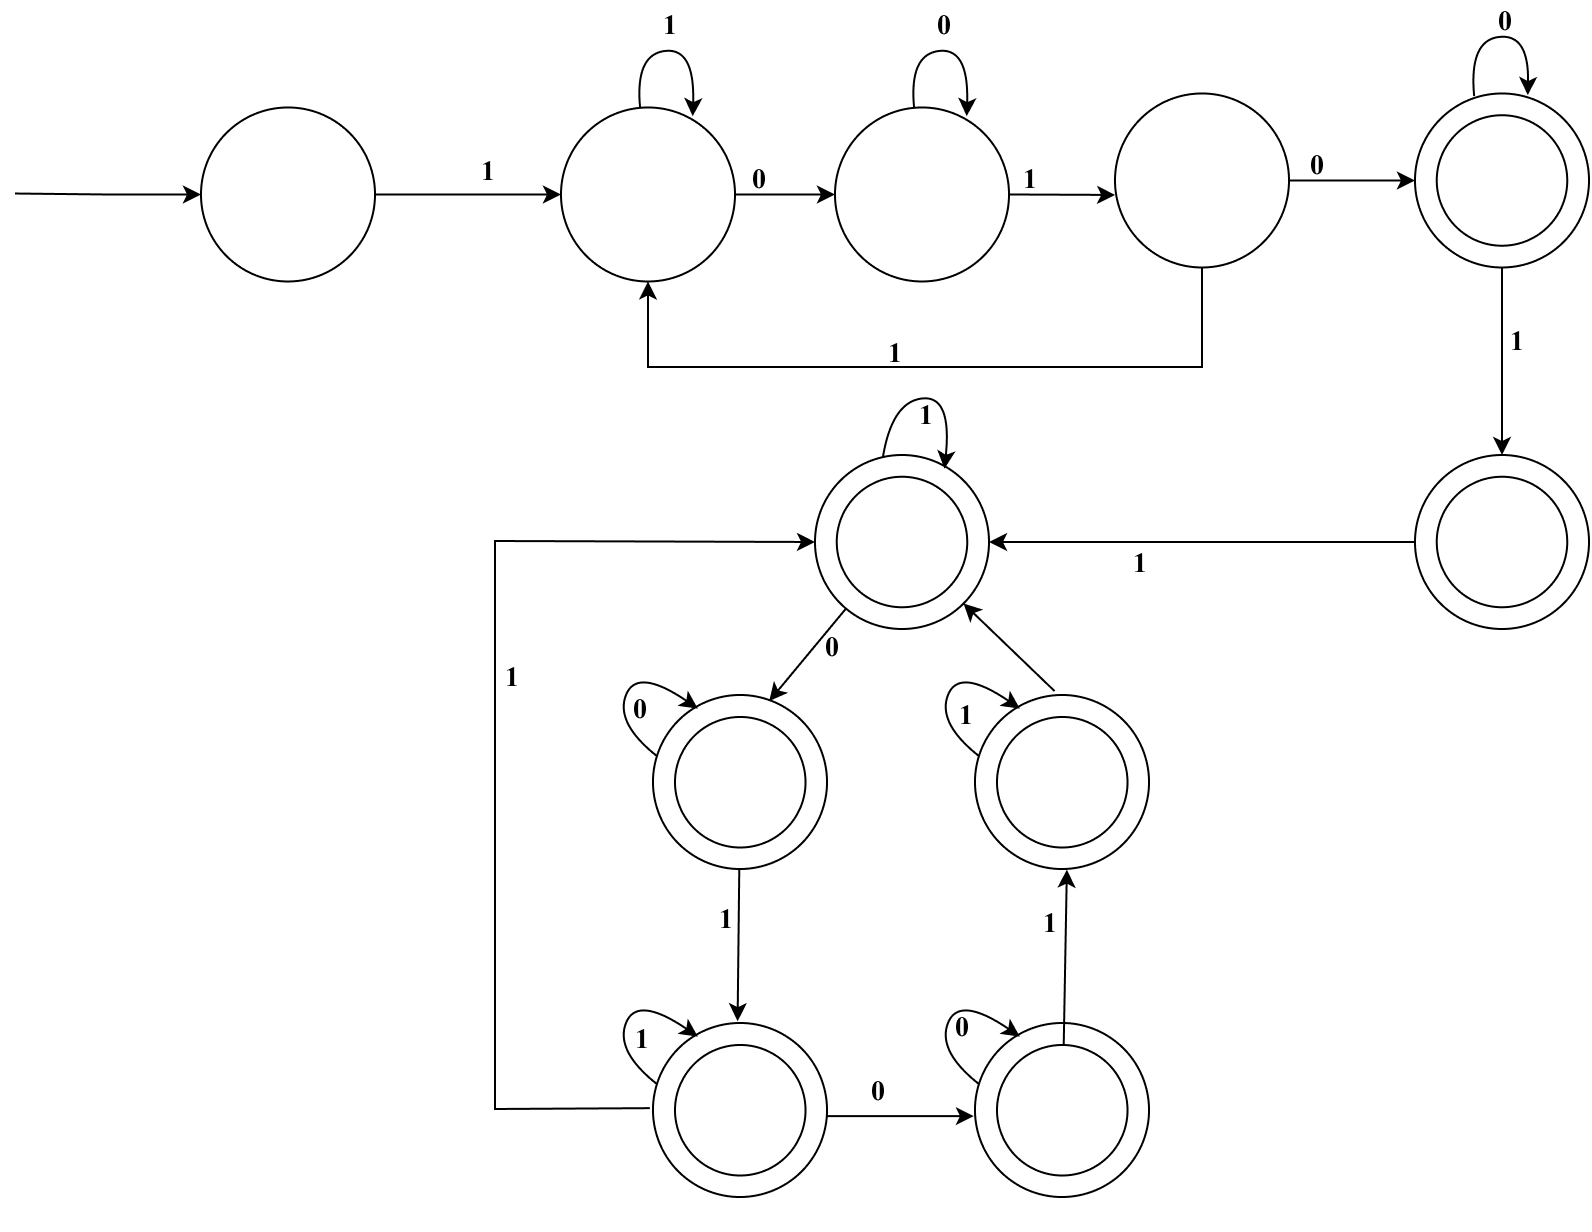
\includegraphics[width=1\textwidth]{q2p1.png}
\end{figure}

نمودار DFA فوق از 3 بخش تشکیل شده است، بخش بالایی که برای ساخت حداقل یک زیررشته‌ی 010 و بخش پایینی که برای جلوگیری از ظاهر شدن زیررشته‌ی 01010 و بخش میانی که برای متصل کردن دو بخش دیگر است.

بخش بالایی DFA را می‌توان با این زبان منظم نشان داد:

\setLTR
$1^+0^+1(10^+1 + 0^+1)$

\setRTL
بخش پایینی DFA را می‌توان با این زبان منظم نشان داد:

\setLTR
$(0^+ + 0^+1^+ + 0^+10^+ + 0^+10^+1)^*$

\setRTL
بخش میانی DFA را می‌توان با این زبان منظم نشان داد:

\setLTR
$1^*$

\setRTL

\textbf{در نتیجه عبارت منظم این زبان برابر است با:}
\setLTR

$1^+0^+1(10^+1 + 0^+1)1^*(0^+ + 0^+1^+ + 0^+10^+ + 0^+10^+1)^*$

\setRTL

\subsection*{بخش ب.}

چون '2' به جز هنگام تشکیل زیررشته "010" بر روی شروط زبان ما تاثیری ندارد، ما می‌توانیم در هر State، عبارت منظم $2^*$ را ورودی بگیریم. پس می‌توانیم بین هر دو کارکتری در عبارت منظم بخش قبلی، $2^*$ را اضافه کنیم. تنها نگرانی ما بابت بخش بالایی DFA است که باید تغییر اساسی کند.

دیدید که با اضافه کردن تنها یک کارکتر به الفای زبان، رشته‌های مورد پذیرش به میزان بسیار زیادی افزایش یافت.



